\documentclass[fleqn]{article}
\usepackage[english]{babel}
\usepackage{a4wide}
\usepackage{latexsym}
\usepackage{times}
%\usepackage{theorem}
\usepackage{url}
\usepackage[final]{graphics}
\usepackage{amsmath,amssymb}
\usepackage{amsfonts}
\usepackage{array}
\usepackage{calc}
\usepackage{xspace}
\usepackage{color}
\usepackage{epsfig}
\usepackage{subfigure}
\usepackage{float}
\usepackage{stmaryrd}
\usepackage{color}
\usepackage{mathtools}
\usepackage{graphicx}
\usepackage{epstopdf}
\usepackage{listings}
\usepackage{color}
\usepackage{booktabs,caption}
%\usepackage[flushleft]{threeparttable}
%\usepackage{amsmath}
\DeclareMathAlphabet{\mathpzc}{OT1}{pzc}{m}{it}
\usepackage{amsthm,amssymb}

\usepackage{amssymb}
\usepackage{graphicx}
\usepackage{epstopdf}
\usepackage{mathtools}

\usepackage{algorithm}
\usepackage[noend]{algpseudocode}

\usepackage{fouriernc}
\pagestyle{plain}
\usepackage{float}
\usepackage[hidelinks]{hyperref}

\usepackage{array}
\newcolumntype{L}[1]{>{\raggedright\let\newline\\\arraybackslash\hspace{0pt}}m{#1}}
\newcolumntype{C}[1]{>{\centering\let\newline\\\arraybackslash\hspace{0pt}}m{#1}}
\newcolumntype{R}[1]{>{\raggedleft\let\newline\\\arraybackslash\hspace{0pt}}m{#1}}

\newtheorem{theorem}{Theorem}
\newtheorem{corollary}{Corollary}
\newtheorem{fact}{Fact}
\newtheorem{hypothesis}{Hypothesis}
\newtheorem{lemma}{Lemma}
\newtheorem{definition}{Definition}

\definecolor{codegreen}{rgb}{0,0.6,0}
\definecolor{codegray}{rgb}{0.5,0.5,0.5}
\definecolor{codepurple}{rgb}{0.58,0,0.82}
\definecolor{backcolour}{rgb}{0.95,0.95,0.92}

\lstdefinestyle{mystyle}{
	backgroundcolor=\color{backcolour},   
	commentstyle=\color{codegreen},
	keywordstyle=\color{magenta},
	numberstyle=\tiny\color{codegray},
	stringstyle=\color{codepurple},
	basicstyle=\footnotesize,
	breakatwhitespace=false,         
	breaklines=true,                 
	captionpos=b,                    
	keepspaces=true,                 
	numbers=left,                    
	numbersep=5pt,                  
	showspaces=false,                
	showstringspaces=false,
	showtabs=false,                  
	tabsize=2
}

\lstset{style=mystyle}


\usepackage{fouriernc}
\pagestyle{plain}

%% macros.tex

\title{\sf Towards BCRT for FPTS \\	
			Best-case response time lower bound}
\author{{\sf H.J. Rivera Verduzco 0977393}\\
{\footnotesize\sl P.O.~Box 513, 5600 MB Eindhoven, The Netherlands}\\
{\footnotesize \sl Email: \tt H.J.Rivera.Verduzco@student.tue.nl}}
%\date{}
\begin{document}
\maketitle

%\begin{abstract}
%\noindent
% Add abstract here %
%\end{abstract}


\section{BCRT lower bound for FPTS}
In this section, we propose a lower bound for the \textit{best-case response time} of a task scheduled under FPTS. In addition, we show that the lower bound that is proposed is tighter than other trivial lower bounds for FPTS.

\subsection{Hypothetical best-case interval for execution of a task $\tau_i$}
\begin{definition} \label{def:hi}
The \textit{hypothetical best-case interval} $HI_i(y,\alpha)$ is defined as the length of the shortest interval $[t_s,t_e)$ in which an amount of time $y \in \mathbb{R}^+$ is available for the execution of $\tau_i$ assuming that all jobs of delaying tasks activated at or after $t_e-\alpha$ are postponed after $t_e$, where $\alpha \in \mathbb{R^+} \cup \{0\}$. Furthermore, all tasks are scheduled under FPPS.
\end{definition}

Note that $HI_i(y,\alpha)$ assumes that all tasks are scheduled under FPPS. Therefore, $HI_i(y,\alpha)$ can be seen as a generalization of the \textit{best-case interval} $BI_i(y)$ defined in \cite{BLM13}, with the addition that jobs of \textit{delaying} tasks activated after or at $t_e-\alpha$ do not influence the amount of time available for task $\tau_i$ in the interval.  Clearly, $HI_i(y,\alpha) = BI_i(y)$ when there are no \textit{delaying} tasks or when $\alpha = 0$. Based on this, we formulate the following theorem. 

%Moreover, note that $\alpha$ is analogous to an activation jitter for all delaying tasks. In order to show this, Figure depicts an optimal instant for FPPS when delaying tasks experience an activation jitter of $\alpha$. As can be seen, this situation is in accordance to Definition \ref{def:hi} because jobs of delaying tasks after $t_e-\alpha$ are postponed after $t_e$.

%Based on the analogous nature between \textit{hypothetical best-case interval} $HI_i(y,\alpha)$ and \textit{best-case interval} $BI_i(y)$ with activation jitter of $\alpha$ for delaying tasks, we can simply use the same analysis for $BI(y)$ to derive $HI_i(y,\alpha)$ restricting the activation jitter for \textit{delaying} tasks to $\alpha$.

\begin{theorem} \label{thrm:hi}
	The \textit{hypothetical best-case interval} $HI_i(y, \alpha)$ in which an amount of time $y\in \mathbb{R^+}$ is available for task $\tau_i$ is given by the largest $x \in \mathbb{R}^+$ satisfying
	\begin{align}
	x = y + \sum\limits_{h:\pi_h > \theta_i} \Big( \Big\lceil  \dfrac{x}{T_h}\Big\rceil -1 \Big)^+  BC_h + \sum\limits_{d:\theta_i \geq \pi_d > \pi_i} \Big( \Big\lceil  \dfrac{x-\alpha}{T_d}\Big\rceil -1 \Big)^+  BC_d,
	\end{align}
	where the notation $w^+$ stands for $\max(w,0)$.
\end{theorem}

\begin{proof}
	Since the only difference between the notion of \textit{hypothetical best-case interval}  $HI_i(y, \alpha)$ and \textit{best-case interval}  $BI_i(y)$ relies on \textit{delaying} tasks, the first part of Theorem \ref{thrm:hi} remains the same for \textit{preemptive} tasks as the analysis of $BI_i(y)$. Hence, we only have to prove that the last term $\sum\limits_{d:\theta_i \geq \pi_d > \pi_i} \Big( \Big\lceil  \dfrac{x-\alpha}{T_d}\Big\rceil -1 \Big)^+  BC_d$ addresses the influence of delaying tasks in the interval $[t_s,t_e)$.
	
	By Definition \ref{def:hi}, jobs of \textit{delaying} tasks activated after time $t_e-\alpha$ do not influence the length $HI_i(y, \alpha)$ of the interval $[t_s,t_e)$. Therefore, we only have to calculate the minimum interference provoked by \textit{delaying} tasks in the interval $[t_s,t_e-\alpha)$. Since this interval has a length of  $HI_i(y, \alpha)-\alpha$, the minimum interference is simply given by  $\sum\limits_{d:\theta_i \geq \pi_d > \pi_i} \Big( \Big\lceil  \dfrac{HI_i(y, \alpha)-\alpha}{T_d}\Big\rceil -1 \Big)^+  BC_d$. Therefore, concluding the proof.
\end{proof}

To calculate $HI_i(y, \alpha)$, we can use an iterative procedure starting with an upper-bound. An appropriate upper-bound to start the iterative procedure is the following.

\begin{lemma}
	An appropriate initial value for the iterative procedure to determine $HI_i(y,\alpha)$ is
	\begin{align}
	HI_i^{(0)}(y,\alpha) = \frac{y}{1-BU_{i-1}}.
	\end{align}
\end{lemma}

\begin{proof}
	Similar to the proof of Lemma 3 in \cite{BLM13}.
\end{proof}

\subsection{Hypothetical shortest response time}
In this section, we first introduce the notion of \textit{hypothetical shortest response time} and subsequently formulate a number of lemmas related with such a notion.

\begin{definition} \label{def:hsrt_def}
%	Assume again that all preemptive tasks of $\tau_i$ are released simultaneously at time $t_p$ and all delaying tasks are released at time $t_p-\alpha$. Furthermore, assume that the jobs of delaying tasks released after or at $t_p-\alpha$ cannot start. Let $\iota_{i,k}$ be a job of $\tau_i$ that completes at $f_{i,k}=t_p$. We define $\Psi_i(\alpha)$ as the \textit{hypothetical shortest response time} of $\iota_{i,k}$ under such assumptions.
The \textit{hypothetical shortest response time} $\Psi_i(\alpha)$ with $\alpha \in \mathbb{R^+} \cup \{0\}$ is defined as the shortest response time of a job $k$ of $\tau_i$ assuming that delaying tasks activated after or at time $f_{i,k}-\alpha$ are postponed after $f_{i,k}$. Furthermore, all tasks are scheduled under FPPS.
\end{definition}

Note that Definition \ref{def:hsrt_def} assumes that all tasks are scheduled under FPPS. Hence, $\Psi_i(\alpha)$ can be seen as a generalization of the \textit{best-case response time} analysis for FPPS and arbitrary deadlines proposed in \cite{BLM13}, with the addition that jobs of \textit{delaying} tasks activated after or at $f_{i,k}-\alpha$ do not influence the response time of $\iota_{i,k}$. Clearly, when there are no \textit{delaying} tasks or when $\alpha = 0$, $\Psi_i(\alpha)$ is the same as the \textit{best-case response time} under FPPS. Recall that the best-case analysis for FPPS investigates whether previous jobs induce blocking in the job experiencing the optimal instant in order to determine its response time. This is done using the notion of \textit{best-case interval} $BI_i(y)$. Based on these observations, we can simply extent the best-case analysis for FPPS with the notion of \textit{hypothetical best-case interval} $HI_i(y,\alpha)$ to determine $\Psi_i(\alpha)$ as follows.

% this definition is similar to the notion of \textit{best-case response time} for FPPS. The only difference is that, for the \textit{hypothetical shortest response time} $\Psi_i(\alpha)$ of a job $k$ of $\tau_i$, delaying tasks activated after or at $f_{i,k}-\alpha$ cannot start. Therefore, in order to determine $\Psi_i(\alpha)$, we can simply extent the analysis for \textit{best-case response time} for FPPS given in \cite{BLM13} to consider the restriction on \textit{delaying} tasks as follows.


\begin{theorem}
	Let all tasks of a task-set $\mathpzc{T}$ be strictly periodic and let $wl_i$ exist. The \textit{hypothetical shortest response time} $\Psi_i(\alpha)$ of a task $\tau_i \in \mathpzc{T}$ is given by
	\begin{align}
	\Psi_i(\alpha) = \max \limits_{1 \leq k \leq wl_i} (HI_i(k \cdot BC_i, \alpha) - (k-1)T_i).
	\end{align}
\end{theorem}

As an example of the \textit{hypothetical shortest response time} $\Psi_i(\alpha)$ of a task $\tau_i$, consider the the task-set with characteristics as describe in Table \ref{tab:ts_Psi_ex}. Note that $\tau_1$ is a \textit{preemptive} task of $\tau_3$, and $\tau_2$ is a \textit{delaying} task. Figure \ref{fig:ex_Psi_alpha} shows a timeline where the \textit{hypothetical shortest response time} $\Psi_3(\alpha)$ for task $\tau_3$ is found when choosing $\alpha=2$. As can be seen, the start of the job of task $\tau_2$ activated at time $t=-2$ is postponed after the completion of the job of $\tau_3$. Furthermore, observe that the job of $\tau_2$ activated at time $t=-6$ can preempt $\tau_3$ because the Definition \ref{def:hsrt_def} assumes that tasks are scheduled under FPPS.

\begin{table}[H]
	\center
	\caption{Task set $\mathpzc{T}_{\ref{tab:ts_Psi_ex}}$.}
	\label{tab:ts_Psi_ex}
	\begin{tabular}{c c c c c | c c }
		\hline 
		& $T_i$ & $C_i$ & $\pi_i$ & $\theta_i$ &  $wl_i$ & $WR_i$ \\ 
		\hline 
		$\tau_1$& 3  & 1  & 3 & 3 &  1 & 1 \\ 
		$\tau_2$& 4  & 1  & 2 & 2 &  3 & 9 \\ 
		$\tau_3$& 12 & 5  & 1 & 2 &  1 & 12 \\
		\hline 
	\end{tabular}
	\small
	\item The \textit{least common multiple} of the periods is 12 and $U^{\mathpzc{T_{\ref{tab:ts_Psi_ex}}}}=1$.
\end{table}

\begin{figure}[H]
	\centering
	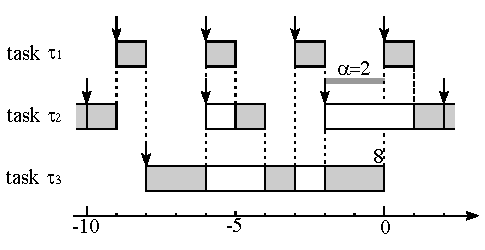
\includegraphics[width=0.55\linewidth]{figures/ex_psi_alpha}
	\caption{A timeline for $\mathpzc{T}_{\ref{tab:ts_Psi_ex}}$ showing the \textit{hypothetical shortest response time} $\Psi_3(2)=8$ for task $\tau_3$.}
	\label{fig:ex_Psi_alpha}
\end{figure}

We now present some corollaries and lemmas related with the notion of \textit{hypothetical shortest response time}. From Definition \ref{def:hsrt_def}, we can conclude that $\alpha$ restricts the number of preemptions that \textit{delaying} tasks can provoke in the \textit{hypothetical shortest response time} of a task. In fact, $\alpha$ can be seen as a forbidden region where \textit{delaying} tasks cannot execute. Therefore, when increasing the value of $\alpha$ in $\Psi_i(\alpha)$, we are increasing the forbidden region of \textit{delaying} tasks, and consequently reducing its influence on the shortest response time of $\tau_i$. From this observation, we formulate the following corollary.

\begin{corollary} \label{lm:monotonicity_Psi_alpha}
	The function $\Psi_i(\alpha)$ describing the \textit{hypothetical shortest response time} of a task $\tau_i$ is a monotonically decreasing function.
\end{corollary}

Since $\Psi_i(\alpha)$ is a monotonically decreasing function, its smallest value is found when $\alpha$ tends to infinity. Clearly, this means that we are simply forbidding the execution of \textit{delaying} tasks completely. Therefore, for this case, the shortest response time of task $\tau_i$ is only influenced by its \textit{preemptive} tasks.

\begin{corollary} \label{hrt_lb}
	A lower bound for the \textit{hypothetical shortest response time} $\Psi_i(\alpha)$ is the shortest hold time $H^{lb}_i$ of $\tau_i$ when considering only preemptive tasks, i.e $\Psi_i(\alpha) \geq H^{lb}_i$ for all $\alpha \in \mathbb{R^+} \cup \{0\}$.
\end{corollary}

%\begin{proof}
%	The proof follows directly from the definition of \textit{hypothetical shortest response time}. Since $\Psi_i(\alpha)$ is always affected by its \textit{preemptive} tasks, the shortest hold time when considering only \textit{preemptive} tasks can never be greater than the shortest response time of a task $\tau_i$.
%\end{proof}

We now introduce a lemma showing a lower bound for the best-case response time of a task scheduled under FPTS.

\begin{lemma} \label{lm:bcrt_lb}
	In FPTS, the \textit{best case response time} $BR_i$ of a task $\tau_i$ is bounded from below by the \textit{hypothetical shortest response time} $\Psi_i(BR_i)$, i.e. $BR_i \geq \Psi_i(BR_i)$.
\end{lemma}

\begin{proof}
	Let $k^{bcrt}$ be a job of $\tau_i$ with $R_{i,k^{bcrt}}=BR_i$. Note that the response time of job $k^{bcrt}$ is not affected by delaying tasks activated after $f_{i,k^{bcrt}} - HT_{i,k^{bcrt}}$ because such tasks cannot preempt $\tau_i$. Now assume that all \textit{delaying} tasks activated after or at time $f_{i,k^{bcrt}} - BR_i$ are postponed after $f_{i,k^{bcrt}}$. Clearly, under this assumption, the new response time $R^\prime_{i,k^{bcrt}}$ of job $k^{bcrt}$ can at most be equal to $BR_i$ because we are reducing the influence of \textit{delaying} tasks in the response time of $k^{bcrt}$. Therefore, $BR_i \geq R^\prime_{i,k^{bcrt}}$.
	
	Recall that $\Psi_i(BR_i)$ is, by definition, the shortest response time of a job $k$ of $\tau_i$ when assuming that delaying tasks activated after or at time $f_{i,k} - BR_i$ are postponed after $f_{i,k}$. Therefore, we can conclude that $R^\prime_{i,k^{bcrt}} \geq \Psi_i(BR_i)$ and consequently $BR_i \geq \Psi_i(BR_i)$
\end{proof}

\subsection{Best-case response time lower bound for FPTS}

\begin{theorem}\label{thm:bcrt_lb}
	Let all tasks of a task-set $\mathpzc{T}$ be strictly periodic and let $wl_i$ exist. A lower bound $BR^{lb}_i$ for the \textit{best-case response time} of a task $\tau_i$ scheduled under FPTS is given by
	\begin{align}
	BR^{lb}_i = \min \limits_{H_i^{lb} \leq \alpha \leq \Psi_i(H_i^{lb})} (\max \{ \alpha, \Psi_i(\alpha) \}),
	\end{align}
	where $H_i^{lb}$ is the shortest hold time of $\tau_i$ when considering only preemptive tasks.
\end{theorem}

\begin{proof}
	We first show that $\min \limits_{H_i^{lb} \leq \alpha \leq \infty} (\max \{ \alpha, \Psi_i(\alpha) \})$ is a lower bound for the \textit{best-case response time} of $\tau_i$. Since we are looking for the minimum result of $\max \{ \alpha, \Psi_i(\alpha)\}$ considering the interval $H_i^{lb} \leq \alpha \leq \infty$, it is sufficient to show that at least for one value of $\alpha$ within that interval the result of $\max \{ \alpha, \Psi_i(\alpha)\}$ is a lower bound for the \textit{best-case response time}. Let $\alpha = BR_i$, clearly this value is in the interval $H_i^{lb} \leq \alpha \leq \infty$. Therefore, we only have to prove that $BR_i \geq \max\{BR_i, \Psi_i(BR_i)\}$. Using Lemma \ref{lm:bcrt_lb}, it holds that $\max\{BR_i, \Psi_i(BR_i)\}=BR_i$; hence, concluding the first part of the proof.
	
	We now want to show that the minimum of $\max \{ \alpha, \Psi_i(\alpha)\}$ can never be found for $\alpha > \Psi_i(H^{lb}_i)$. In order to prove this, first note that by choosing $\alpha = H_i^{lb}$ and using Corollary \ref{hrt_lb}, it holds that $\max\{H^{lb}_i, \Psi_i(H^{lb}_i)\}=\Psi_i(H^{lb}_i)$. Since for any value of $\alpha > \Psi_i(H^{lb}_i)$ the result of $\max \{ \alpha, \Psi_i(\alpha)\}$ is always greater than $\Psi_i(H^{lb}_i)$, we conclude that the minimum can never be found for such values; therefore, a proper upper bound for $\alpha$ is $\Psi_i(H^{lb}_i)$.
\end{proof}

\subsection{Tightness of $BR^{lb}_i$}
A trivial lower bound for the \textit{best-case response time} of a task $\tau_i$ scheduled under FPTS is the shortest hold-time $H^{lb}_i$ of such a task when ignoring \textit{delaying} tasks, i.e. when considering only preemptive tasks. We want to show that the lower bound $BR^{lb}_i$ described in Theorem \ref{thm:bcrt_lb} is tighter than $H^{lb}_i$ for many cases.

We first show that $BR^{lb}_i$ is always larger than $H^{lb}_i$. From Lemma \ref{lm:bcrt_lb}, we know that $\Psi_i(\alpha) \geq H^{lb}_i$, we therefore derive that $\max \{ \alpha, \Psi_i(\alpha) \} \geq  H^{lb}_i$. Hence, $BR^{lb}_i \geq H^{lb}_i$ in general.

We now show the cases where $BR^{lb}_i$ is tighter than $H^{lb}_i$, i.e. when $BR^{lb}_i > H^{lb}_i$. Firstly, note that for $\alpha >  H^{lb}_i$, it holds that $\max \{ \alpha, \Psi_i(\alpha) \}) >  H^{lb}_i$. In addition, when $\Psi(H^{lb}_i) > H^{lb}_i$, it also holds that $\max \{ \alpha, \Psi_i(\alpha) \} >  H^{lb}_i$ for $\alpha =  H^{lb}_i$. Therefore, we conclude that for the cases where $\Psi(H^{lb}_i) > H^{lb}_i$, the lower bound $BR^{lb}_i$ presented in Theorem \ref{thm:bcrt_lb} is tighter than $H^{lb}_i$.

\subsection{An algorithm for computing the BCRT lower bound}

Theorem 2 gives a lower bound for the \textit{best-case response time} of a task $\tau_i$. However, since $\alpha \in \mathbb{R^+} \cup \{ 0 \}$ is a continuous variable, the set of values where $H_i^{lb} \leq \alpha \leq \Psi_i(H_i^{lb})$ holds may be infinite. In order to solve this, Algorithm 1 shows a procedure to derive the lower bound of the \textit{best-case response time}  presented in Theorem 2 for a task $\tau_i$. Nevertheless, instead of trying all possible values of $\alpha$ in the interval $H_i^{lb} \leq \alpha \leq \Psi_i(H_i^{lb})$, Algorithm 1 starts with $\alpha=H_i^{lb}$ and only increases $\alpha$ in discrete steps that can decrease the result of $\max \{ \alpha, \Psi_i(\alpha)\}$. If the result of $\max \{ \alpha, \Psi_i(\alpha)\}$ starts increasing instead of decreasing, the algorithm terminates and the minimum is found. Note that this is a good point to stop the algorithm because $\Psi_i(\alpha)$ is a monotonically decreasing function. Therefore, if the result of the expression $\max \{ \alpha, \Psi_i(\alpha)\}$ starts increasing when increasing $\alpha$, it means that $\alpha$ becomes the dominant term in $\max \{ \alpha, \Psi_i(\alpha)\}$, and the result of $\Psi_i(\alpha)$ will continue increasing.

%\footnote{Note: Probably to show that this is indeed a good point to stop the algorithm, I have to explain first (in a possible proof) that $\Psi_i(\alpha)$ is a monotonically decreasing function}

The procedure in Algorithm 1 first assigns to $\alpha$ the hold time of $\tau_i$ when considering only preemptive tasks. In Line 3, $\max \{ \alpha, \Psi_i(\alpha)\}$ with the initial value of $\alpha$ is chosen as an initial candidate for the best-case lower bound value $BR_i^{lb}$. Furthermore, in case that $BR^{lb}_i$ is higher than $\alpha$, it means that it is possible to increase $\alpha$ hopefully leading to a reduction in the best-case lower bound. Hence, Lines 5-7 increase the value of $\alpha$. More precisely, the job $k^{tight}$ of task $\tau_i$ that induces some blocking on the start time of the job experiencing the \textit{hypothetical shortest response time} is determined in Line 5. Moreover, Lines 6 and 7 determine the time the forbidden region $\alpha$ of delaying tasks should be increased in order to prevent job $k^{tight}$ from inducing some blocking. At this point, the result of $\max \{ \alpha, \Psi_i(\alpha)\}$ with the new value of $\alpha$ is assigned to $BR^{lb}_i$ only if it is smaller than its current value. This is expressed in Line 8. Finally, if the new value of $\alpha$ is still smaller than the new value of $BR^{lb}_i$, the procedure is repeated. Otherwise, the algorithm terminates.


%if the new value of $\alpha$ exceeds the current $BR^{lb}_i$, then the result of $\max \{ \alpha, \Psi_i(\alpha)\}$ can only increase the value of $BR^{lb}_i$; hence, the algorithm terminates. Otherwise, it assigns the result of $\max \{ \alpha, \Psi_i(\alpha)\}$ to $BR^{lb}_i$ in Line 9 and the process is repeated. 

Table \ref{tab:terminology_br} shows an overview of the variables used in Algorithm 1.


%  lines 7 to 9 push the activation for the delaying tasks in order to allow to reduce $BR^{lb}_i$ in the next iteration.
%
%$BR^{lb}_i$ is initialized with some upper bound. A lower bound candidate is derived in line 5 using a similar approach as for the \textit{best-case response time} analysis for FPPS. The purpose of the outer max is to make sure that $BR^{lb}_i$ is at least the same as the activation of delaying tasks $AD_i$. In case that $BR^{lb}_i$ is higher than $AD_i$, lines 7 to 9 push the activation for the delaying tasks in order to allow to reduce $BR^{lb}_i$ in the next iteration. More precisely, the job $k^{tight}$ of task $\tau_i$ that induces some delay on the start time of the job experiencing the optimal instant is determined in line 7. Moreover, lines 8 and 9 determine the time the activation of delaying tasks should be pushed at an earlier moment in order to prevent job $k^{tight}$ from inducing some blocking. At this point, if the new value of $AD_i$ exceeds the current $BR^{lb}_i$, then it is not beneficial to push the activation of delaying tasks to reduce the \textit{best-case response time}; hence, the algorithm terminates.

\begin{table}[H]
	\center
	\caption{Terminology.}
	\label{tab:terminology_br}
	\begin{tabular}{|c | p{11cm}|}
		\hline
		Name & Descriptions \\ 
		\hline 
		\hline
		$BR^{lb}_i$& Lower bound of the best-case response time of $\tau_i$.\\
		\hline
		$\alpha$& Length of the forbidden region of \textit{delaying} tasks. It is assumed that \textit{delaying} jobs activated in this region are postponed.\\
		\hline
		$k^{tight}$& Job of $\tau_i$ inducing some blocking on the start time of the job experiencing the \textit{hypothetical shortest response time}.\\
		\hline
		$DI_i$& Length of the time interval between the activation of the job $k^{tight}$ of $\tau_i$ and the start of the forbidden region of \textit{delaying} tasks with length $\alpha$.\\
		\hline 
	\end{tabular}
	%\small
	%\item Add extra caption.
\end{table} 

%\begin{algorithm}[H]
%	\caption{Algorithm to derive a lower bound for the \textit{best-case response time} of a task $\tau_i$.}\label{euclid}
%	\begin{algorithmic}[1]
%		\Procedure{\textit{bcrtLowerBound}}{$\mathpzc{T}$,$i$}
%		\State $\alpha \gets$ a lower bound on the hold time of $\tau_i$;
%		\While {$\Psi_i(\alpha) > \alpha$}
%		\State $k^{tight} \gets$ the smallest $k$ with $1 \leq k \leq wl_i$ that leads to $\Psi_i(\alpha)$;
%		\State $DI_i \gets \Psi_i(\alpha) + (k^{tight}-1)T_i - \alpha$;
%		\State $\alpha \gets \min \limits_{d:\theta_i \geq \pi_d > \pi_i} (DI_i \mod T_d) + \alpha$
%		\EndWhile{\textbf{end while}}
%		\State \Return $\alpha$; 
%		\EndProcedure
%	\end{algorithmic}
%\end{algorithm}

\begin{algorithm}[H]
	\caption{Algorithm to derive a lower bound for the \textit{best-case response time} of task $\tau_i$.}\label{euclid}
	\begin{algorithmic}[1]
		\Procedure{\textit{bcrtLowerBound}}{$\mathpzc{T}$,$i$}
		\State $\alpha \gets$ shortest hold time of $\tau_i$ when considering only preemptive tasks;
		\State $BR^{lb}_i \gets \max\{\alpha, \Psi_i(\alpha) \}$;
		\While {$ \alpha < BR^{lb}_i$}
		\State $k^{tight} \gets$ the smallest $k$ with $1 \leq k \leq wl_i$ that leads to $BR^{lb}_i$;
		\State $DI_i \gets BR^{lb}_i + (k^{tight}-1)T_i - \alpha$;
		\State $\alpha \gets \min \limits_{d:\theta_i \geq \pi_d > \pi_i} (DI_i \mod T_d) + \alpha$;
		\State $BR^{lb}_i \gets \min \{BR^{lb}_i, \max\{\alpha, \Psi_i(\alpha) \}\}$;
		%\If {$BR^{lb}_i > \alpha$}
		%\State $BR^{lb}_i \gets \max\{\alpha, \Psi_i(\alpha) \}$;
		%\EndIf {\textbf{end if}}
		\EndWhile{\textbf{end while}}
		\State \Return $BR^{lb}_i$; 
		\EndProcedure
	\end{algorithmic}
\end{algorithm}

\subsection{An example}
Consider the set of tasks $\mathpzc{T}_{\ref{tab:ts_example}}$ with characteristics as described in Table $\ref{tab:ts_example}$. We will apply Algorithm 1 to derive a lower bound $BR^{lb}_4$ for the \textit{best-case response time} of task $\tau_4$. Figure \ref{fig:bcrt_lb_ex1} shows an example of how each variable of the algorithm would be represented in a timeline for $\mathpzc{T}_{\ref{tab:ts_example}}$ after the first iteration. Furthermore, note that tasks $\tau_1$ and $\tau_2$ are \textit{preemptive} tasks of $\tau_4$, whereas $\tau_3$ is a \textit{delaying} task. As can be seen, $\alpha^{(0)}=22$ represents the initial value of $\alpha$, and it is initially equal to the hold time of the last job of $\tau_4$. Furthermore, the job of $\tau_4$ activated at time $t=560$ denoted as $k^{tight}$ is the one that leads to the \textit{hypothetical response time} of $\Psi_4(\alpha^{(0)})=36$, and subsequently to $BR_4^{lb(0)}=36$. 

Note that, in Figure \ref{fig:bcrt_lb_ex1}, it is possible to increase the forbidden region of \textit{delaying} task $\tau_3$ in order to allow more space for the execution of $\tau_4$. Therefore, the algorithm increments $\alpha$ till an activation of $\tau_3$ coincides with the activation of job $k^{tight}$ of $\tau_4$. This time increment can be calculated as $(DI_4 \mod T_3)$, and it leads to $\alpha^{(1)}=26$. Note that, at this point, $BR^{lb (0)}_4$ is still larger than $\alpha^{(1)}$; hence, the algorithm will recalculate $BR^{lb}_4$.

%Based on this, the algorithm then determines the value $AD^{(1)}_4=26$ that would allow to push the phase of $\phi_4$ further in order to reduce the \textit{best-case response time} of $\tau_4$. Note that $BR^{lb (1)}_4$ is larger than $AD^{(1)}_4$; hence, the algorithm will continue with the next iteration.

\begin{table}[H]
	\center
	\caption{Task set $\mathpzc{T}_{\ref{tab:ts_example}}$.}
	\label{tab:ts_example}
	\begin{tabular}{c c c c c | c c c}
		\hline 
		& $T_i$ & $WC_i=BC_i$ & $\pi_i$ & $\theta_i$ &  $wl_i$ & $WR_i$ & $BR_i$\\ 
		\hline 
		$\tau_1$& 35 & 5  & 4 & 4 &  1 & 5 & 5\\ 
		$\tau_2$& 35 & 5  & 3 & 3 &  1 & 10 & 5\\ 
		$\tau_3$& 50 & 20 & 2 & 2 &  2 & 62 & 20\\ 
		$\tau_4$& 70 & 22 & 1 & 2 &  5 & 66 & 27\\
		\hline 
	\end{tabular}
	\small
	\item The \textit{least common multiple} of the periods is 350 and $U^{\mathpzc{T_{\ref{tab:ts_example}}}}=1$.
\end{table}

\begin{figure}[H]
	\centering
	\includegraphics[width=1\linewidth]{figures/bcrt_lb_ex1.PNG}
	\caption{Example after the first iteration of $bcrtLowerBound(\mathpzc{T}_{\ref{tab:ts_example}},4)$. }
	\label{fig:bcrt_lb_ex1}
\end{figure}

Figure \ref{fig:bcrt_lb_ex2} shows the timeline for the second iterations of $bcrtLowerBound(\mathpzc{T}_{\ref{tab:ts_example}},4)$. As can be seen, the activations of the \textit{delaying} task $\tau_3$ was pushed to an earlier moment in time, allowing to decrease the \textit{hypothetical response time} $\Psi_4(\alpha^{(1)})=22$ of the last job. At this point $BR^{lb(1)}_4 = \alpha^{(1)} = 26$; hence, the algorithm terminates because there is no previous job restricting the response time of the last job of $\tau_4$. Therefore, $BR^{lb}_4 = 26$ is a proper lower bound for the \textit{best-case response time} of $\tau_4$.


\begin{figure}[H]
	\centering
	\includegraphics[width=1\linewidth]{figures/bcrt_lb_ex2.PNG}
	\caption{Example after the second iteration of $bcrtLowerBound(\mathpzc{T}_{\ref{tab:ts_example}},4)$. }
	\label{fig:bcrt_lb_ex2}
\end{figure}


\begin{thebibliography}{10}
	\bibitem{BLM13}
	R.J. Bril, J.J. Lukkien, and R.H. Mak.
	Best-case response times and jitter analysis of real-time tasks with arbitrary deadlines.
	In Proc. 21st International Conference on Real-Time Networks and Systems (RTNS), ACM, pp. 193-202, October 2013.
	
\end{thebibliography}

\end{document}

